% Generated by code/needham.py -- do not edit by hand.
\definecolor{qocA}{rgb}{0.00,0.45,0.70}
\definecolor{qocB}{rgb}{0.90,0.60,0.00}
\definecolor{qocC}{rgb}{0.00,0.62,0.45}
\definecolor{qocD}{rgb}{0.80,0.40,0.00}
\definecolor{qocE}{rgb}{0.80,0.60,0.70}
\definecolor{qocF}{rgb}{0.35,0.70,0.90}
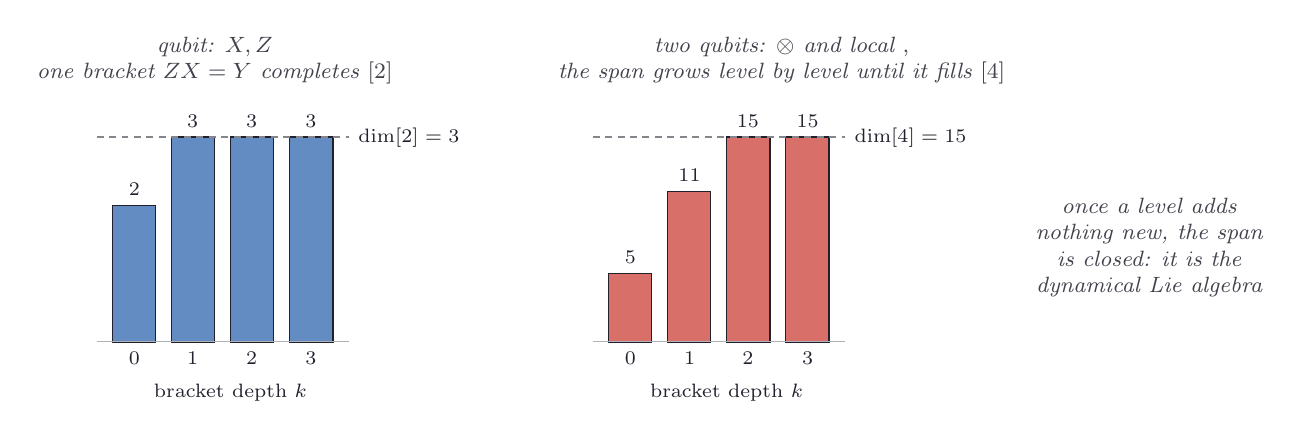
\begin{tikzpicture}[ink/.style={line width=0.9pt, ndInk}, faint/.style={line width=0.4pt, ndInk!35}, dashedink/.style={line width=0.5pt, ndInk!55, dash pattern=on 2.5pt off 2pt}, vec/.style={->, >=stealth, line width=1.2pt}, note/.style={font=\footnotesize\itshape, text=ndInk!85, align=center}, pointer/.style={->, >=stealth, line width=0.4pt, ndInk!60, shorten >=2pt, shorten <=1pt}, dot/.style={circle, fill=ndInk, inner sep=0pt, minimum size=3.4pt}, wash/.style={fill=ndSky, fill opacity=0.55}, every node/.style={text=ndInk}]
\definecolor{ndInk}{rgb}{0.13,0.13,0.18}
\definecolor{ndPaper}{rgb}{0.99,0.96,0.88}
\definecolor{ndSky}{rgb}{0.84,0.91,0.98}
\definecolor{ndRose}{rgb}{0.98,0.86,0.84}
\definecolor{ndBlue}{rgb}{0.13,0.36,0.66}
\definecolor{ndRed}{rgb}{0.78,0.20,0.16}
\definecolor{ndGold}{rgb}{0.88,0.62,0.10}
\definecolor{ndGreen}{rgb}{0.18,0.52,0.30}
\fill[ndBlue, fill opacity=0.7] (0.00,0) rectangle (0.55,1.733);
\draw[ink, line width=0.5pt] (0.00,0) rectangle (0.55,1.733);
\node[font=\scriptsize, above] at (0.28,1.733) {2};
\node[font=\scriptsize, below] at (0.28,0) {0};
\fill[ndBlue, fill opacity=0.7] (0.75,0) rectangle (1.30,2.600);
\draw[ink, line width=0.5pt] (0.75,0) rectangle (1.30,2.600);
\node[font=\scriptsize, above] at (1.02,2.600) {3};
\node[font=\scriptsize, below] at (1.02,0) {1};
\fill[ndBlue, fill opacity=0.7] (1.50,0) rectangle (2.05,2.600);
\draw[ink, line width=0.5pt] (1.50,0) rectangle (2.05,2.600);
\node[font=\scriptsize, above] at (1.77,2.600) {3};
\node[font=\scriptsize, below] at (1.77,0) {2};
\fill[ndBlue, fill opacity=0.7] (2.25,0) rectangle (2.80,2.600);
\draw[ink, line width=0.5pt] (2.25,0) rectangle (2.80,2.600);
\node[font=\scriptsize, above] at (2.52,2.600) {3};
\node[font=\scriptsize, below] at (2.52,0) {3};
\draw[faint] (-0.20,0) -- (3.00,0);
\draw[dashedink] (-0.20,2.600) -- (3.00,2.600) node[right, font=\scriptsize] {$\dim\liesu[2]=3$};
\node[font=\scriptsize] at (1.50,-0.65) {bracket depth $k$};
\fill[ndRed, fill opacity=0.7] (6.30,0) rectangle (6.85,0.867);
\draw[ink, line width=0.5pt] (6.30,0) rectangle (6.85,0.867);
\node[font=\scriptsize, above] at (6.58,0.867) {5};
\node[font=\scriptsize, below] at (6.58,0) {0};
\fill[ndRed, fill opacity=0.7] (7.05,0) rectangle (7.60,1.907);
\draw[ink, line width=0.5pt] (7.05,0) rectangle (7.60,1.907);
\node[font=\scriptsize, above] at (7.33,1.907) {11};
\node[font=\scriptsize, below] at (7.33,0) {1};
\fill[ndRed, fill opacity=0.7] (7.80,0) rectangle (8.35,2.600);
\draw[ink, line width=0.5pt] (7.80,0) rectangle (8.35,2.600);
\node[font=\scriptsize, above] at (8.07,2.600) {15};
\node[font=\scriptsize, below] at (8.07,0) {2};
\fill[ndRed, fill opacity=0.7] (8.55,0) rectangle (9.10,2.600);
\draw[ink, line width=0.5pt] (8.55,0) rectangle (9.10,2.600);
\node[font=\scriptsize, above] at (8.83,2.600) {15};
\node[font=\scriptsize, below] at (8.83,0) {3};
\draw[faint] (6.10,0) -- (9.30,0);
\draw[dashedink] (6.10,2.600) -- (9.30,2.600) node[right, font=\scriptsize] {$\dim\liesu[4]=15$};
\node[font=\scriptsize] at (7.80,-0.65) {bracket depth $k$};
\node[note, anchor=south] at (1.3,3.15) {qubit: $X,Z$\\ one bracket $\comm ZX=Y$ completes $\liesu[2]$};
\node[note, anchor=south] at (8.5,3.15) {two qubits: $\sigz\otimes\sigz$ and local $\sigx,\sigy$\\the span grows level by level until it fills $\liesu[4]$};
\node[note, anchor=west] at (11.6,1.2) {once a level adds\\ nothing new, the span\\ is closed: it is the\\ dynamical Lie algebra};
\end{tikzpicture}
